\chapter{Introduction}
\label{chapter_introduction}
%% Start the actual chapter on a new page.
\newpage

\noindent 
\dropcap{S}{peciation} is the process that creates new species,
connecting all of life to one shared common ancestor. It is a process
that has resulted in the millions of species on Earth nowadays, 
as well as in the many species that have gone extinct.
Some speciation events that gave rise to extant species, 
happened earlier than others,
from hundreds of millions of years ago (so-called 'long-enduring species',
or, informally, 'living fossil') 
to more recent ones. See figure \ref{fig:long_enduring_and_young_species} 
shows an example of each.

\begin{figure}[H]
  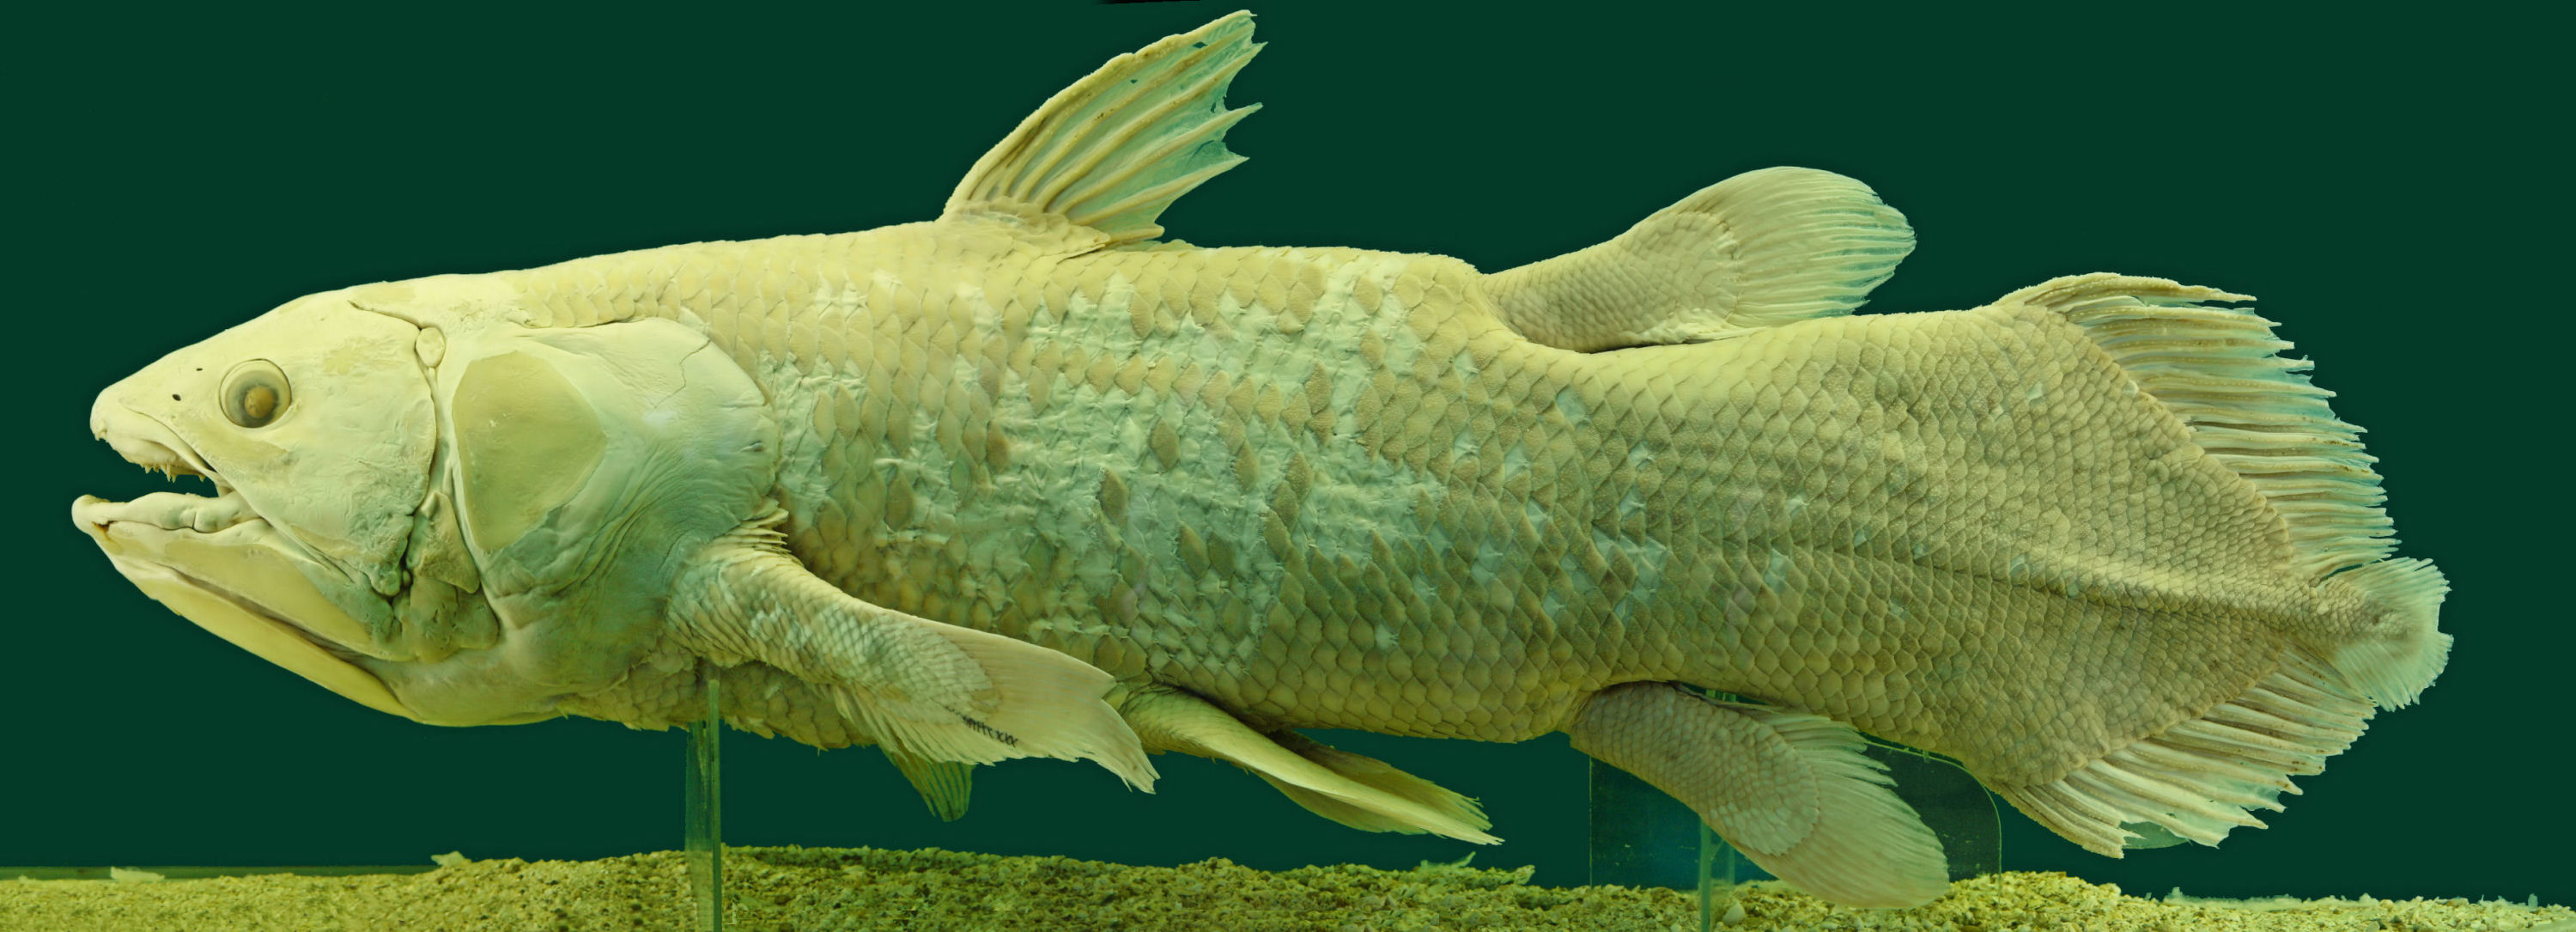
\includegraphics[width=0.80\textwidth]{latimeria_chalumnae.jpg}
  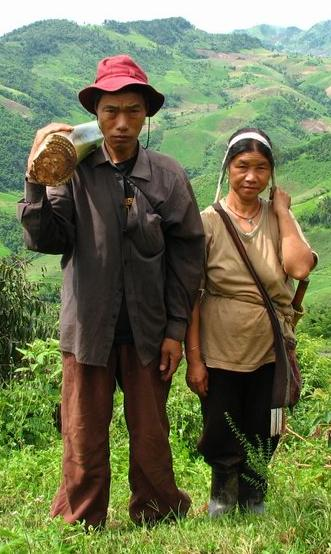
\includegraphics[width=0.18\textwidth]{homo_sapiens.jpg}
  \caption{
    An long-enduring species (left) and a young species (right).
    The species at the left is a preserved specimen of \textit{Latimeria chalumnae}, 
    estimated to exist for hundreds of millions of year.
    The species at the right is the \textit{Homo sapiens}, 
    existing for around a third of a million years.
  }
  \label{fig:long_enduring_and_young_species}
\end{figure}

A first very basic question within the field of biology,
is to ask which species are closest related to
one another. 
[MAKE STRONGER CASE HERE]
If you think that's an easy question, try to apply it, 
for example, on the 8 crocodilian pictures in figure \ref{fig:crocodialians}.
You may come up with one or more pairs of hypothesized closest-related species,
but you will probably get stuck on which ancestors of these pairs
are most closely related. Note that doing the other way around, to use
morphology to classify species, is tricky: how to decide when the morphology 
between two specimens is different enough to classify these as two species?

\begin{figure}[H]
  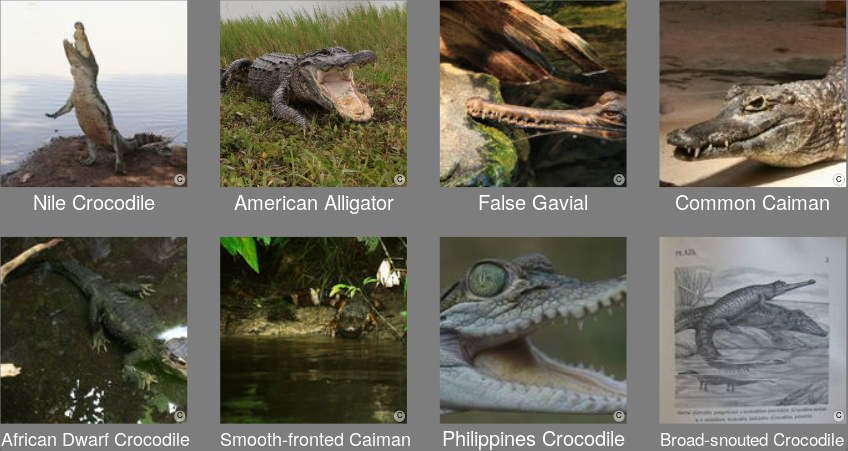
\includegraphics[width=1.0\textwidth]{crocodilians.png}
  \caption{
    Eight members of the order of crocodilians
  }
  \label{fig:crocodialians}
\end{figure}

The second very basic biological question, is to 
ask \emph{when} these speciation events took place.
This question cannot be answered based on morphologies of the present-day
species alone, because morphology is a complex trait, and the pace at
which morphology changes in time is unknown or unpredictable.

This second question can be answered by
using a classical approach, 
by using the morphology of fossils.
This approach can only be used if the species \emph{can} fossilize,
and those fossils are found in multiple points in time.
Even if this is the case, there are caveats. Using morphology on
extinct species is even trickier, as species change their appearance in time.
Also an imaginary time machine would not help us out:
we could try to determine the number of species in each timepoint,
but that would only work if we could confidently define what a
species is. We cannot, because speciation is usually a gradual process.

This second question can also be answered 
using a modern approach, 
by using the DNA sequences of extant species,
as shown, for example, in figure \ref{fig:alignment}.
Because DNA is inherited from parent to offspring
and changes through times, it carries each species' 
evolutionary histories within it.
The point in time when a species speciates is
marked by the two daughter species having seperate mutations
from that moment on.
Due to this, we can easily find closest related species 
by measuring the similarity in DNA sequences.
If we know how frequent mutations occur, we can already
do a rough estimation of when the speciation event took place.
In reality, DNA sequences of different species 
varies in length, due to insertions and deletions in genetic sequences,
but in the simulation studies in this thesis, we will ignore this.

\begin{figure}[H]
  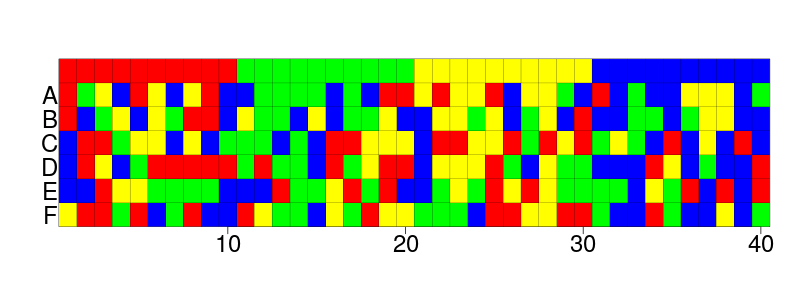
\includegraphics[width=0.8\textwidth]{alignment_40_with_root.png}
  \caption{
    A 40-nucleotide DNA alignment of six hypothetical species. The species
    are named A to and including F. 
    The four colors denote the four different nucleotides,
    in which the red color resembles adenine, yellow depicts cytosine, 
    green is for guanine, and blue resembles thymine. The top
    row shows the (artificial) root sequence, which is usually unknown.
  }
  \label{fig:alignment}
\end{figure}

Using the DNA sequences of extant species to answer our biological questions,
however, is a complex topic. For starters, there are multiple 
ways to do so, like bootstrapping, 
jack-knifing, parsimony, maximum likelihood and more.
A conveniently simple approach is to use UPGMA [DEFINE AND EXPLAIN], which answer our biological
questions, in the form of a phylogeny.


\begin{figure}[H]
  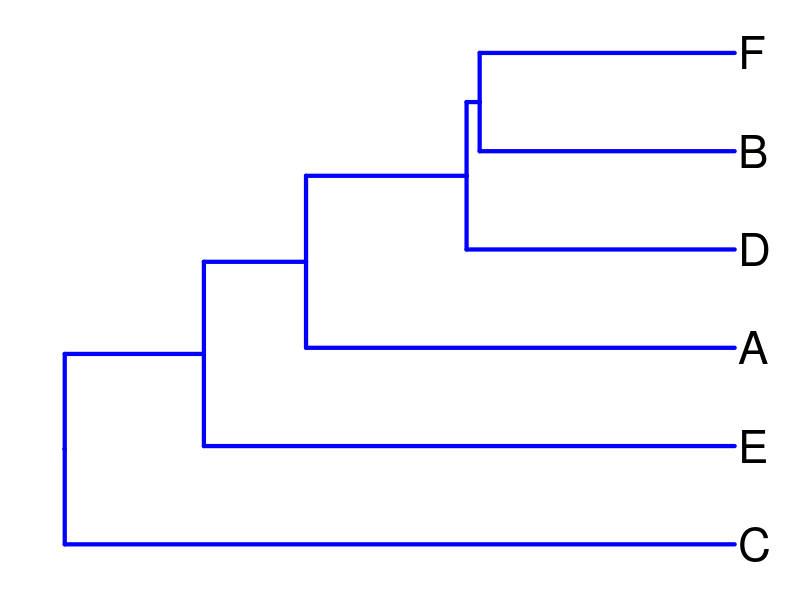
\includegraphics[width=0.4\textwidth]{phylogeny_40_upgma.png}
  \caption{
    Phylogeny created from the alignment in figure \ref{fig:alignment} 
    using UPGMA. 
    This method is irrelevant in the context of this thesis.
  }
  \label{fig:phylogeny_upgma}
\end{figure}

Figure \ref{fig:phylogeny_upgma} shows a phylogeny, [ASSUME MORE KNOWLEDGE]
created from the alignment 
in figure \ref{fig:alignment} using one such methodology.
It shows the six hypothetical species and their evolutionary 
relationships. Going from left to right, we travel through time from 
the past to the present. 
The leftmost vertical line indicates the first speciation event, 
which gave rise to the first two ancestral species. 
This first split in the tree is called the crown,
the moment in time this occurred is called the crown age. [CHANGE TONE TO SCIENTIFIC JOURNAL]

The problem with phylogenies is, 
that it is impossible to go out in the field and measure one, 
as they depict which species lived when \emph{in the past}.
Instead, we \emph{construct} phylogenies. For example,
the phylogeny in figure \ref{fig:phylogeny_upgma}, how well
does match the true phylogeny? \textbf{That question, is the main question of this 
thesis: how well can we construct a
phylogeny from an alignment?} What is the error we
make when we construct a phylogeny?

Answering this research question is, at first glance, easy: 
1. simulate a true phylogeny.
2. simulate an alignment that follows that phylogeny.
3. construct a phylogeny from that alignment.
4. measure the difference between the true and constructed phylogeny.
This workflow is depicted in figure \ref{fig:research_workflow_single}.
All steps, however, are more complex than just this.

%%%%%%%%%%%%%%%%%%%%%%%%%%%%%%%%%%%%%%%%%%%%%%%%%%%%%%%%%%%%%%%%%%%%%%%%%%%%%%%%%%%%%%
% Figure 1
%%%%%%%%%%%%%%%%%%%%%%%%%%%%%%%%%%%%%%%%%%%%%%%%%%%%%%%%%%%%%%%%%%%%%%%%%%%%%%%%
\begin{figure}[H]
  \centering
  \resizebox {0.8\columnwidth} {!} {
    \begin{tikzpicture}[->,>=stealth',shorten >=1pt,auto,node distance=4cm, semithick]   
    \tikzstyle{every state}=[]
    \node[state] (A) [rectangle] {
      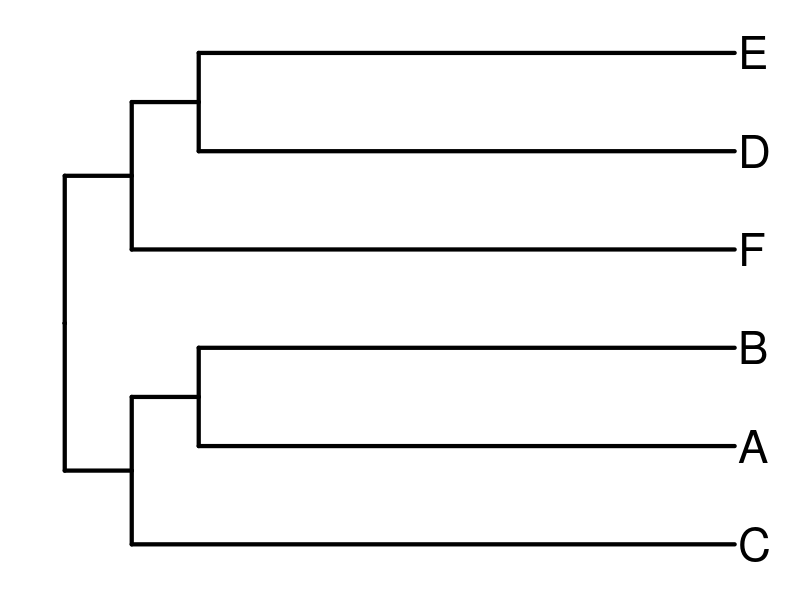
\includegraphics[width=0.3\textwidth]{phylogeny.png}
    };   
    \node[state] (AL) [above left=-0.25cm and -0.25cm of A, fill=white] {
      1
    };   
    \node[state] (B) [below of = A, rectangle] {
      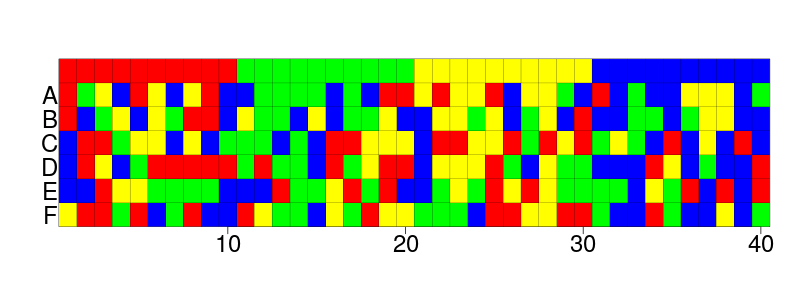
\includegraphics[width=0.6\textwidth]{alignment_40_with_root.png}
    };   
    \node[state] (BL) [above left=-0.25cm and -0.25cm of B, fill=white] {
      2
    };   
    \node[state] (C) [below of = B, rectangle] {
      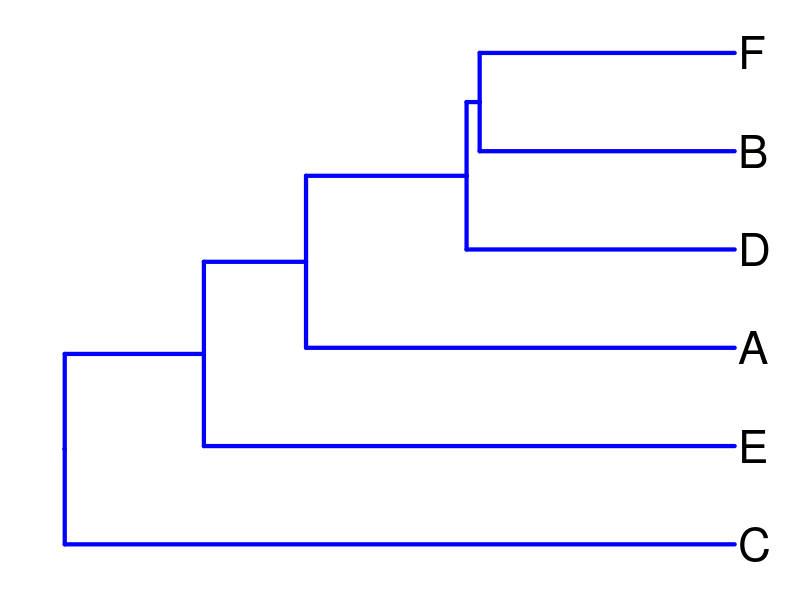
\includegraphics[width=0.3\textwidth]{phylogeny_40_upgma.png}
    };   
    \node[state] (CL) [above left=-0.25cm and -0.25cm of C, fill=white] {
      3
    };
    \node[state] (D) [below of = C, rectangle] {
      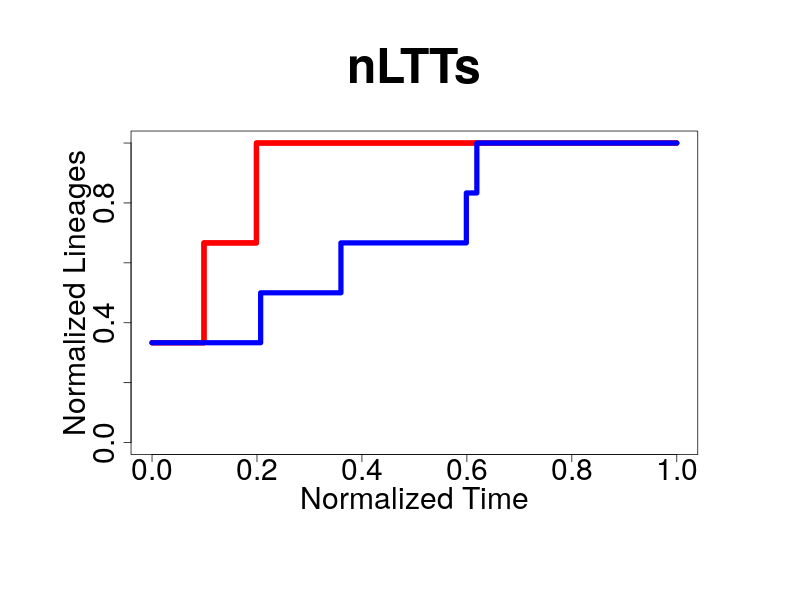
\includegraphics[width=0.4\textwidth]{nltt_40_true_and_upgma.png}
    };   
    \node[state] (DL) [above left=-0.25cm and -0.25cm of D, fill=white] {
      4
    };
    \path 
      (A) edge [anchor = south] node {} (B)
      (B) edge [anchor = south] node {} (C)
      (A) edge [bend left = 80, anchor = east] node {} (D)
      (C) edge [anchor = south] node {} (D)
    ; 
    \end{tikzpicture}
  }
  \caption{
    (Simplified) method to answer the research question of this thesis:
    1. simulate a true phylogeny. 
    2. simulate an alignment that follows that phylogeny. 
    3. construct a phylogeny from that alignment.
    4. compare the true and constructed phylogeny.
  }
  \label{fig:research_workflow_single}
\end{figure}
%%%%%%%%%%%%%%%%%%%%%%%%%%%%%%%%%%%%%%%%%%%%%%%%%%%%%%%%%%%%%%%%%%%%%%%%%%%%%%%%

Constructing a phylogeny from an alignment is the step that
gets most attention in this thesis, as it is also the most complex
one. Unlike the methods described earlier, 
we do not construct one single phylogeny, 
but we construct a distribution of multiple phylogenies.
Within this distribution of multiple phylogenies, the phylogenies
that are more likely, will be present more often.
This method is called Bayesian phylogenetics, in which we use
a Bayesian approach to create phylogenies based on genetics.

%%%%%%%%%%%%%%%%%%%%%%%%%%%%%%%%%%%%%%%%%%%%%%%%%%%%%%%%%%%%%%%%%%%%%%%%%%%%%%%%%%%%%%
% Figure 1
%%%%%%%%%%%%%%%%%%%%%%%%%%%%%%%%%%%%%%%%%%%%%%%%%%%%%%%%%%%%%%%%%%%%%%%%%%%%%%%%
\begin{figure}[H]
  \centering
  \resizebox {0.8\columnwidth} {!} {
    \begin{tikzpicture}[->,>=stealth',shorten >=1pt,auto,node distance=4cm, semithick]   
    \tikzstyle{every state}=[]
    \node[state] (A) [rectangle] {
      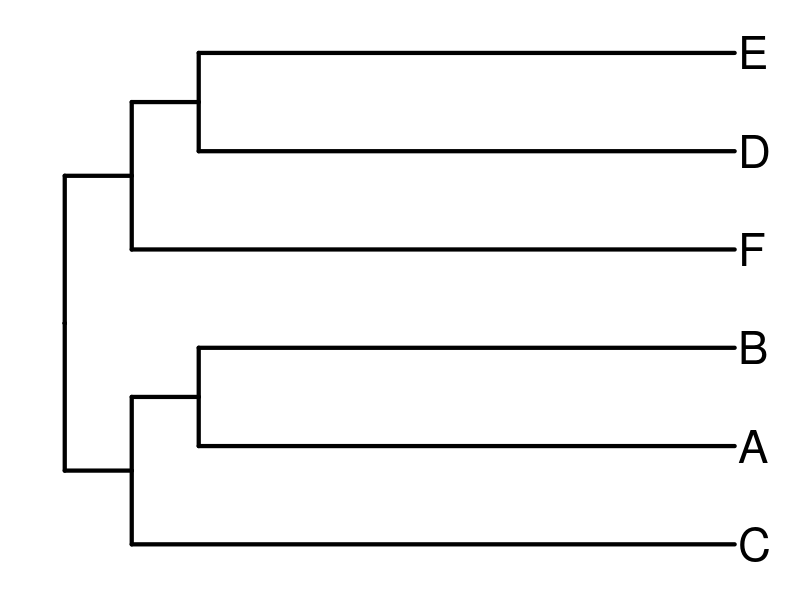
\includegraphics[width=0.3\textwidth]{phylogeny.png}
    };   
    \node[state] (AL) [above left=-0.25cm and -0.25cm of A, fill=white] {
      1
    };   
    \node[state] (B) [below of = A, rectangle] {
      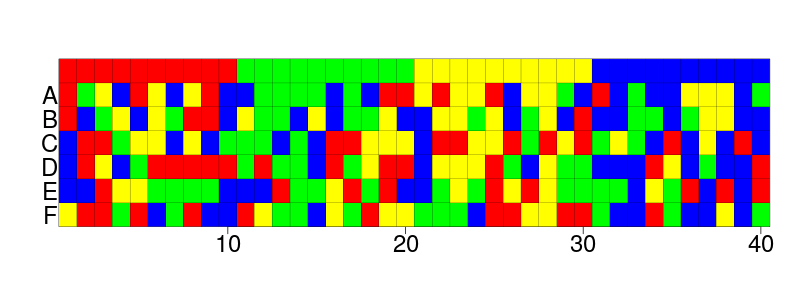
\includegraphics[width=0.6\textwidth]{alignment_40_with_root.png}
    };   
    \node[state] (BL) [above left=-0.25cm and -0.25cm of B, fill=white] {
      2
    };   
    \node[state] (C) [below of = B, rectangle] {
      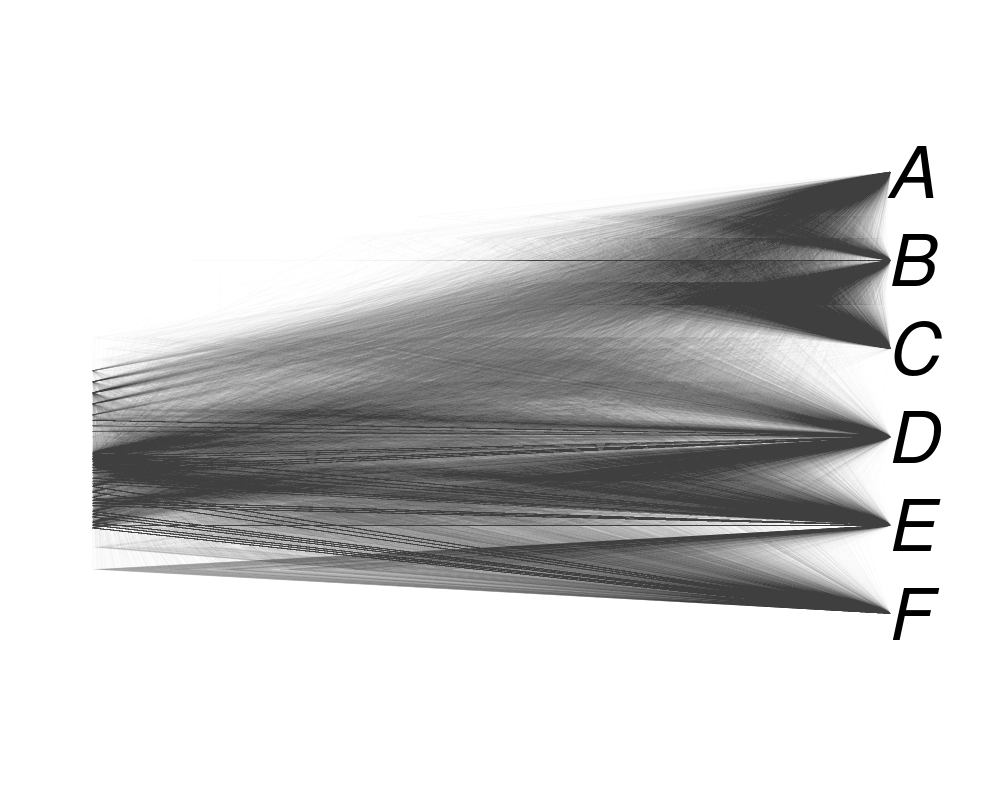
\includegraphics[width=0.3\textwidth]{densitree_40.png}
    };   
    \node[state] (CL) [above left=-0.25cm and -0.25cm of C, fill=white] {
      3
    };
    \node[state] (D) [below of = C, rectangle] {
      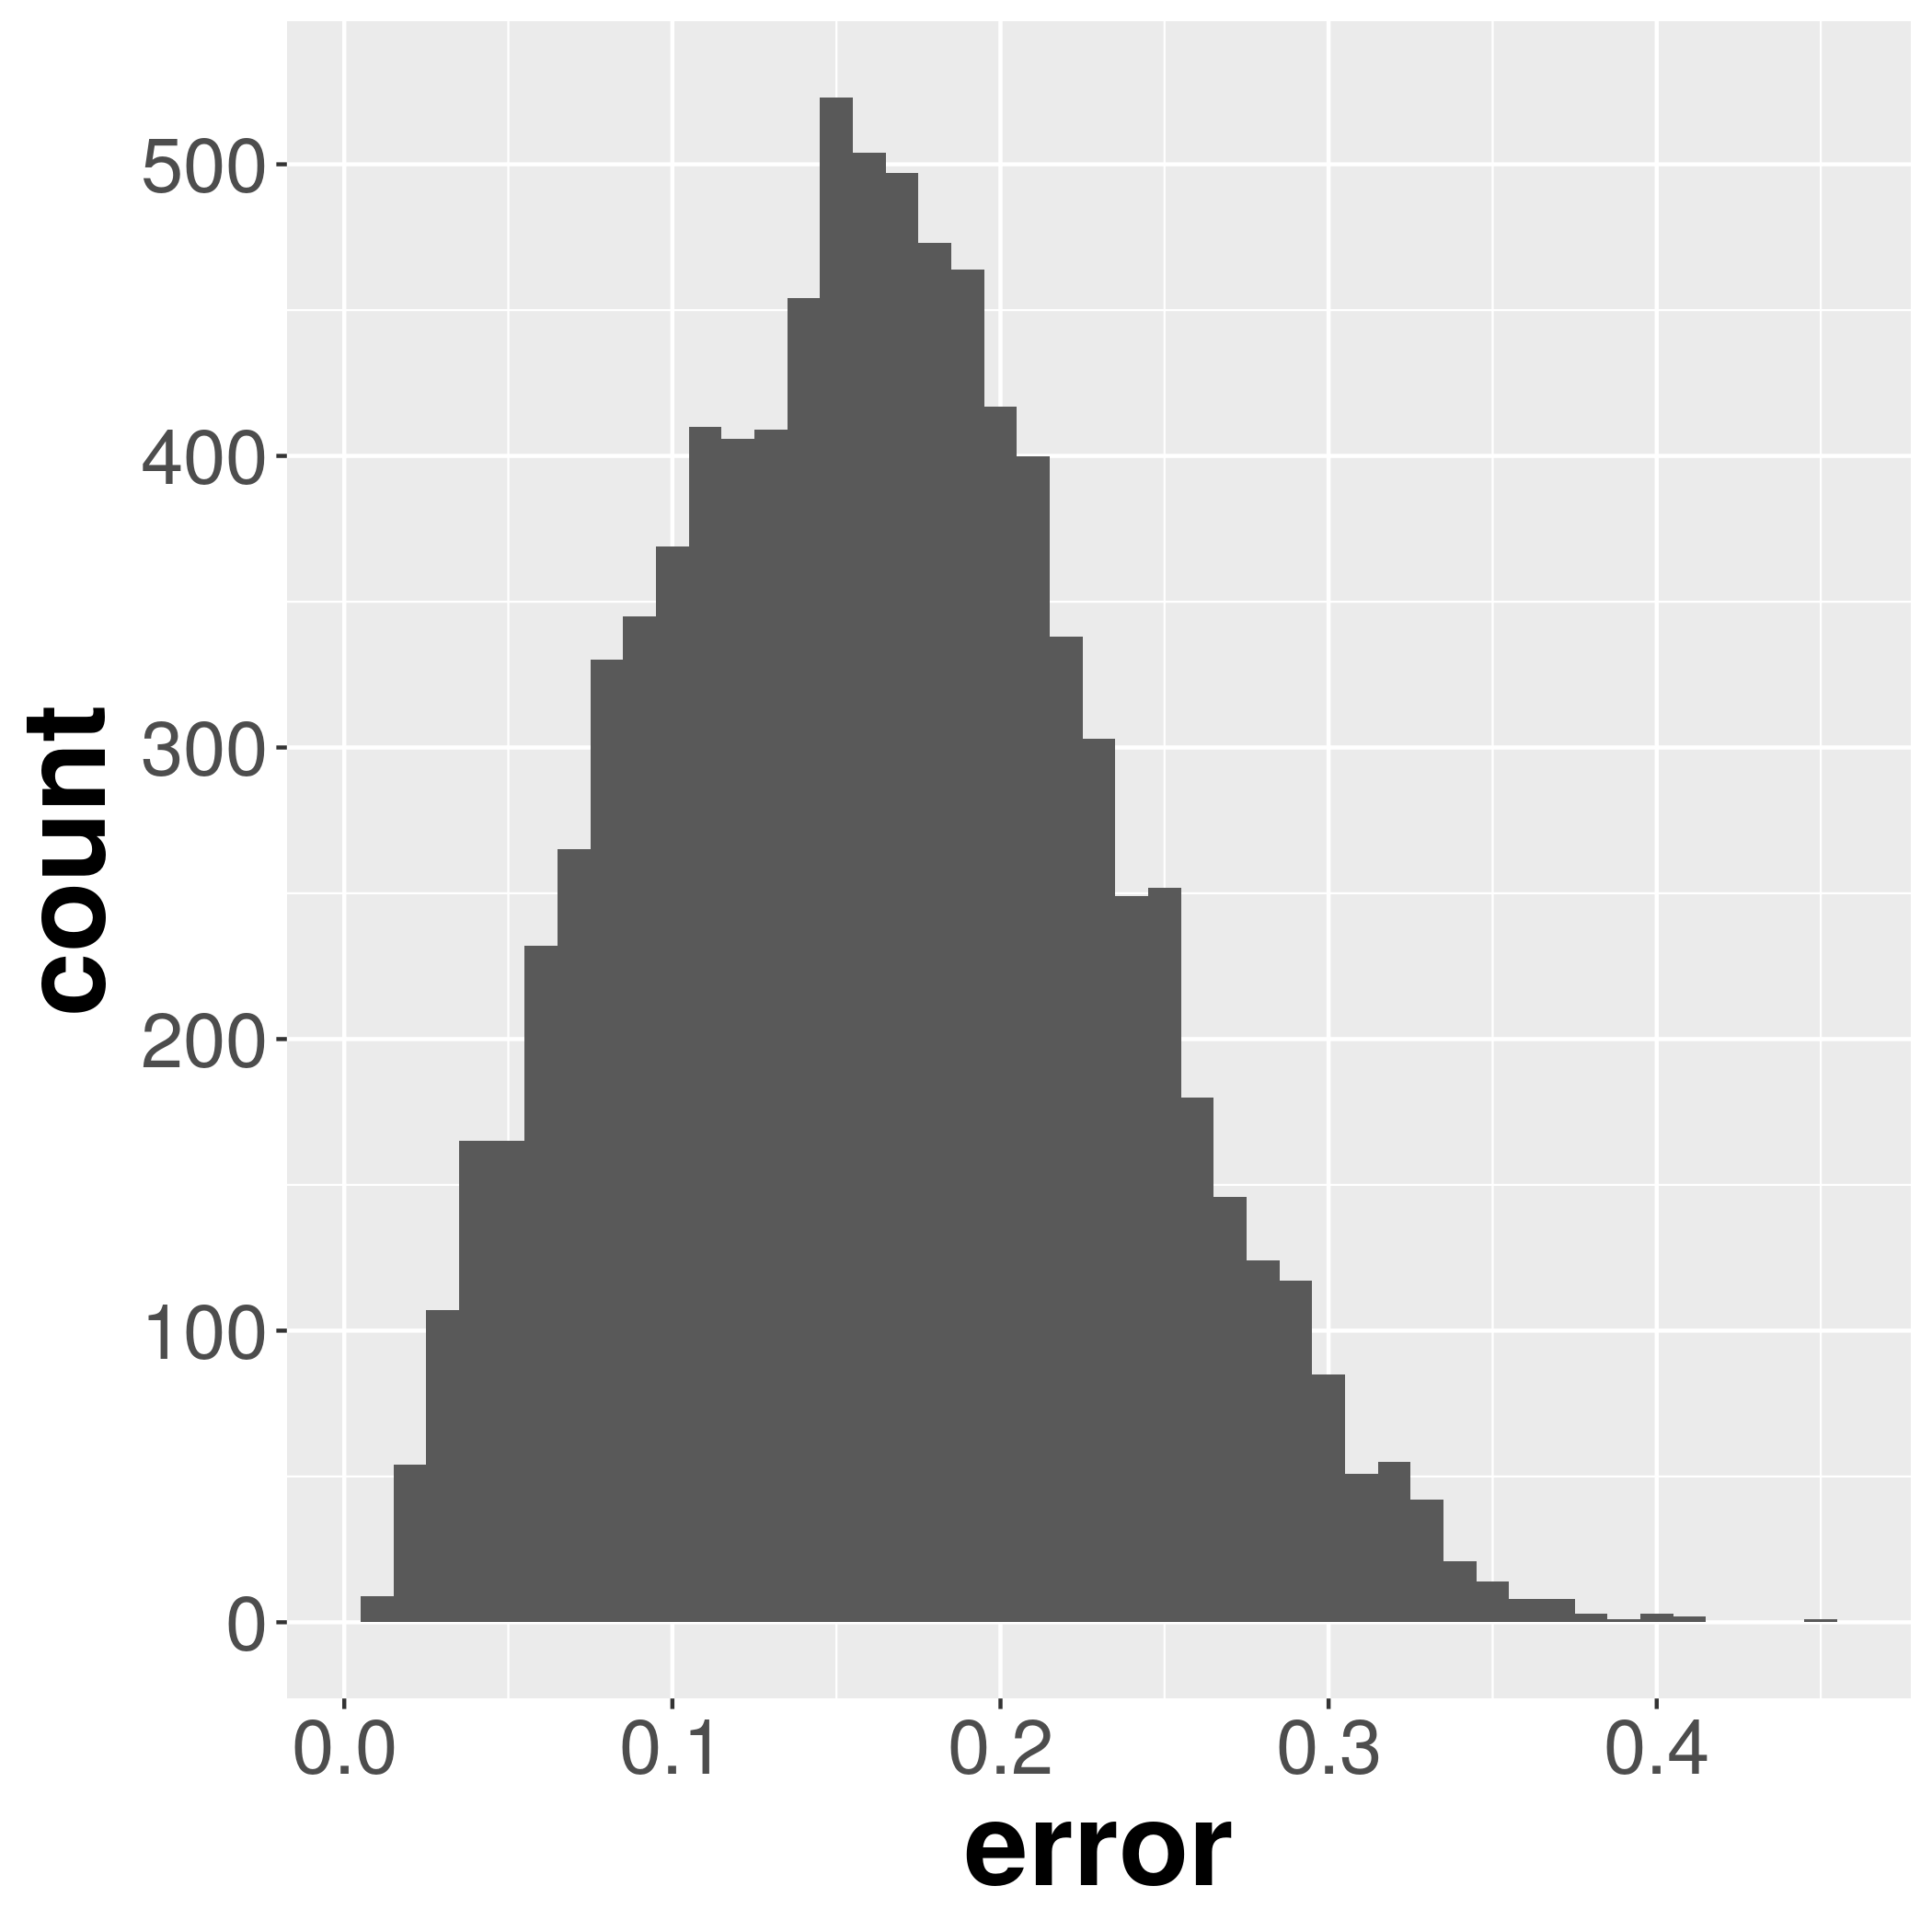
\includegraphics[width=0.29\textwidth]{errors_40.png}
    };   
    \node[state] (DL) [above left=-0.25cm and -0.25cm of D, fill=white] {
      4
    };
    \path 
      (A) edge [anchor = south] node {} (B)
      (B) edge [anchor = south] node {} (C)
      (A) edge [bend left = 80, anchor = east] node {} (D)
      (C) edge [anchor = south] node {} (D)
    ; 
    \end{tikzpicture}
  }
  \caption{
    Method to answer the research question of this thesis:
    1. simulate a true phylogeny. 
    2. simulate an alignment that follows that phylogeny. 
    3. infer a distribution of phylogenies from that alignment.
    4. compare the true phylogenies with the inferred phylogenies.
  }
  \label{fig:research_workflow}
\end{figure}
%%%%%%%%%%%%%%%%%%%%%%%%%%%%%%%%%%%%%%%%%%%%%%%%%%%%%%%%%%%%%%%%%%%%%%%%%%%%%%%%

With Bayesian inference, we need an alignment and our model assumptions to
infer phylogenies.
The model assumptions specify what we assume to be true regarding how
the alignment came to be. For example, we can assume that 1. the true
phylogeny had a constant speciation and extinction rate, 2. the
mutation rate is constant and equal for all species and 3. all
mutations between nucleotides are equally likely. 

[ALP: This is the point at the heart of these thesis, right? In order to infer phylogenetic topology and divergence times we need to assume a certain model for speciation and extinction. You need to build the case for why the current model used may not be appropriate and why more complex models may be required. You really need to delve into the 1) literature on speciation, to discus the biological/geographical/environmental mechanisms underlying speciation and our latest understanding of how speciation works 2) literature on modelling diversification, highlighting how there have been major advances in modelling different modes and tempo of speciation when estimating diversification but not (surprisingly) when infering trees. You need to highlight the logical inconsistency of this and why it could be severely problematic - if we assume certain speciation modes when infering trees does this bias what speciation mode we would infer from that tree??  ]
The result of a Bayesian inference, is -to be precise- a posterior
disribution of jointly-inferred phylogenies and model parameter estimates,
simply called 'posterior' in this thesis.
The way such a posterior is generated assures that more likely phylogenies 
are present more often. 
This distribution of phylogenies shows the
(un)certainty of the inference.
For example, the posterior phylogenies in figure \ref{fig:research_workflow},
panel 3, show a high degree of uncertainty, as the
inferred phylogenies vary widely in shape. The posterior correctly
suggests two clades (ABC and DEF), but does not confidently show
the two most related taxa (AB and DE). We can already make 
the rough claim that, would the phylogeny in panel 1 
in figure \ref{fig:research_workflow} depict
a true phylogeny, we make a big error in its inference.

To be able to do the phylogentic inference needed for the rest of this
thesis, I developed an R package to do so, which
is discussed in chapter 2. Because a Bayesian inference can be set up in
many ways, the greatest asset of that package is that it gives a
consistent grammar to express each setup. Additionally, the R package allows
to run Bayesian inference from the command-line, which is essential for
the theoretical studies in this thesis.

If we can measure the error we make in our inference, 
we can try and improve the inference. 
One way to improve it, is to use a better inference model.
Ideally, we would use the same inference model that gave rise to
the true phylogeny and alignment, but, alas, 
we (usually) do not know that model.
We do not know that model, because we do not know the
model that nature used: the
processes that cause speciation are possibly many, and 
the mechanisms of each are unknown and/or debatable.
[ALP: but you need to go into this in detail to build the case for why the existing models are unlikely to be sufficient or at least why it is important to explore potentially more realistic models]
Due to this, we'll have to resort to the many phylogentic models 
to explain the DNA (RNA, protein, morphological and fossil) data best.

There are plenty of phylogentic models, ranging from simplistic to
very complex. The most popular models make it into our
phylogenetic programs (which, in turn, may make these models even
more popular), which I will define as 'standard models'.
When empiricist build a phylogenetic tree from their
painstakingly acquired DNA alignment, they pick their favorite standard
model or use an algorithm to select one. The empiricist assumes that the
standard models are good enough for his/her cause.

The standard models, however, make some assumptions that will not hold
in all biological cases. 
[ALP: expand on this to explain what the standard model is and what assumptions they make] This will increase the error we make in
our inference. But will that error be profound enough to reject using
a standard model? 

To be able to determine the impact of using a standard phylogentic
model, when we know the biological process in more complex than it
assumes, me and Giovanni Laudanno developed an R package 
to quantify the error we make due to this mismatch, which is described
in chapter 3.

[ALP: Great! this is what i was looking for. You need much more of this kind of stuff. There are other scenarios you might want to discuss e.g. barriers that result in multiple species being isolated simultaneously like when habitat layers move up and down mountains during ice ages species get isolated on the tops or in the valleys.]
One assumption of all standard models is that speciation event happen
independently, that is, there are never two speciation events at the same time. 
There are biological scenario's in which may say
this is false: when a habitat is split up, 
due to a geological barrier, this will result in two 
species communities. The change from one to two communities is likely
to affect both communities and trigger a speciation event in both
communities. The inference error of ignoring co-occurring speciation is quantified by
me and Giovanni Laudanno in chapter 4.

[ALP: you need to provide a lot more information and discussion here - why does speciation take time? Does it always take time or can it be instantaneous? Are there examples of clades that you can use to illustrate your arguments? You need to delve  into the theory and empirical evidence of speciation here to make a compelling case for why a protracted model that at least allows speciation to occur gradually is needed. Again, highlight how this has been implemented to infer speciation dynamics from tree but oddly the models used to infer the tree in the first place ignore this. ]
Another assumption of all standard models is that speciation event happen
instantaneously, that is, when there is a speciation event, the two species
are immediatly recognized as such. We know that speciation takes
time. 
The inference error of ignoring this fact is quantified by
me in chapter 5.

In chapter 6, I show which conclusions can be drawn from these chapters

\references{dissertation}

\subsection{Photo attribution}

Figure \ref{fig:long_enduring_and_young_species},
the left image,
\href{https://en.wikipedia.org/wiki/File:Latimeria_Chalumnae_-_Coelacanth_-_NHMW.jpg}{Preserved specimen of chalumnae}
by Alberto Fernandez Fernandez
is licensed under \href{https://creativecommons.org/licenses/by-sa/3.0/deed.en}{CC BY-SA 3.0}.
the image at the right,
\href{https://commons.wikimedia.org/wiki/File:Akha_cropped_hires.JPG}{Akha couple in northern Thailand}
by Weltenbummler84
is licensed under \href{https://creativecommons.org/licenses/by-sa/2.0/de/deed.en}{CC BY-SA 2.0 DE}.

For figure \ref{fig:crocodialians},
the selection of these eight images was done by 
\href{https://www.onezoom.org/life.html/@Crocodylia=195672\#x1602,y148,w4.1516}{OneZoom}.
These images, from top-left to bottom-row, row-first:
% 1
\href{http://media.eol.org/content/2018/04/11/13/61270_orig.jpg}{Nile Crocodile}
by Marco Schmidt
is licensed under \href{http://creativecommons.org/licenses/by-sa/3.0}{CC-BY-SA 3.0}.
% 2
\href{https://www.flickr.com/photos/nasakennedy/14159295507}{American Alligator}
by NASA Kennedy.
% 3
\href{http://media.eol.org/content/2014/10/06/10/58393_orig.jpg}{False Gavial}
by Yinan Chen
is marked as being in the public domain.
% 4
\href{http://media.eol.org/content/2012/06/13/05/87714_orig.jpg}{Common Caiman}
by Michael Wolf
is licensed under \href{http://creativecommons.org/licenses/by/2.5}{CC-BY 2.5}.
% 5
\href{http://media.eol.org/content/2013/06/11/03/12146_orig.jpg}{African Dwarf Crocodile}
by Staycoolandbegood
is marked as being in the public domain.
% 6
\href{http://media.eol.org/content/2013/11/25/21/58484_orig.jpg}{Smooth-fronted Caiman}
by Whaldener Endo
is licensed under \href{http://creativecommons.org/licenses/by-sa/4.0}{CC-BY-SA 4.0}
% 7
\href{http://media.eol.org/content/2013/06/11/03/06619_orig.jpg}{Phillipines Crocodile}
by Vanderploeg
is marked as being in the public domain.
% 8
\href{http://media.eol.org/content/2014/10/06/16/93746_orig.jpg}{Board-snouted Crocodile}
by Hadonos
is Marked as being in the public domain.
